\section{\aimTwo}

\note{Active learning, also known as optimal experiment design, is a field that concerns itself with estimating statistical models with as few experiments as possible. Existing literature deals mostly with cases where we can choose exactly what to sample; for example, OED has been deployed in the design of guide RNAs for CRISPR gene editing. In our case, we can only choose the stimuli not the entire brain state. Thus, a causal model will be essential for the penultimate application: brain state replay. }

\begin{frame}{\qTwo}
    \textbf{Hypothesis:} Model-based optimal experiment design will reduce underdetermination
    \begin{itemize}
        \item We can choose optimal optogenetic stimuli to maximally reduce model parameter uncertainty
        \item This can be potentially be done online
        \item We can evaluate how well we have done by attempting to track a brain trajectory
    \end{itemize}
\end{frame}

\begin{frame}{Active learning}{Best to ask for category of which image? }
    \vspace*{\fill}
    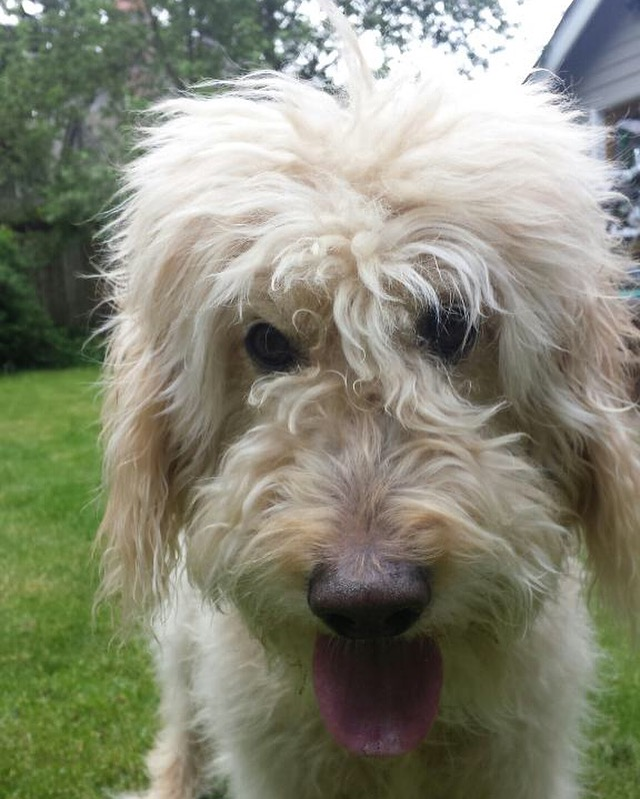
\includegraphics[width=0.31\textwidth]{media/benji.jpg}\nakedfootnote<2>{Mom \& Dad. \emph{personal correspondence}. 2016.}
    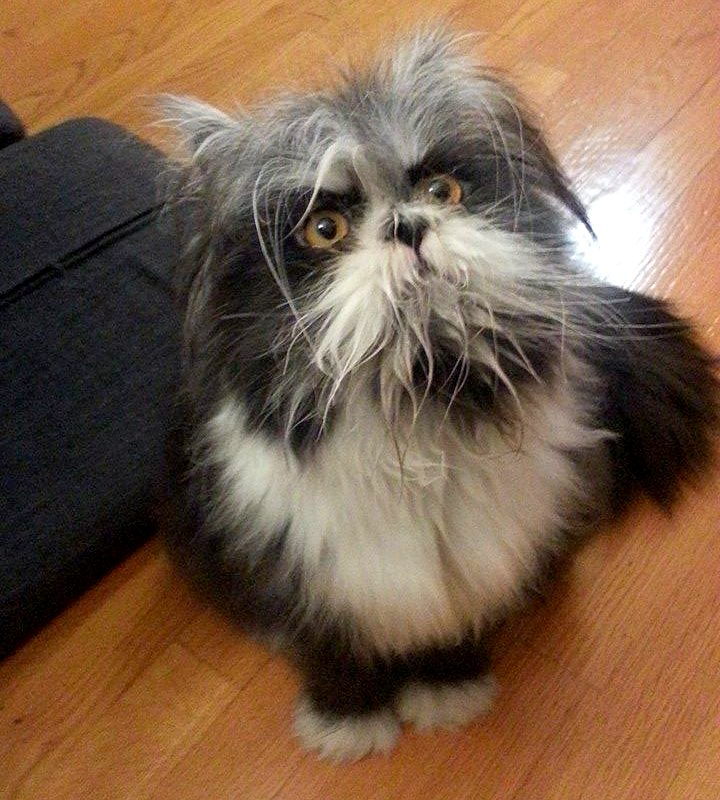
\includegraphics[width=0.31\textwidth]{media/dog-cat}\nakedfootnote<2>{Instagram:atchoumthecat}
    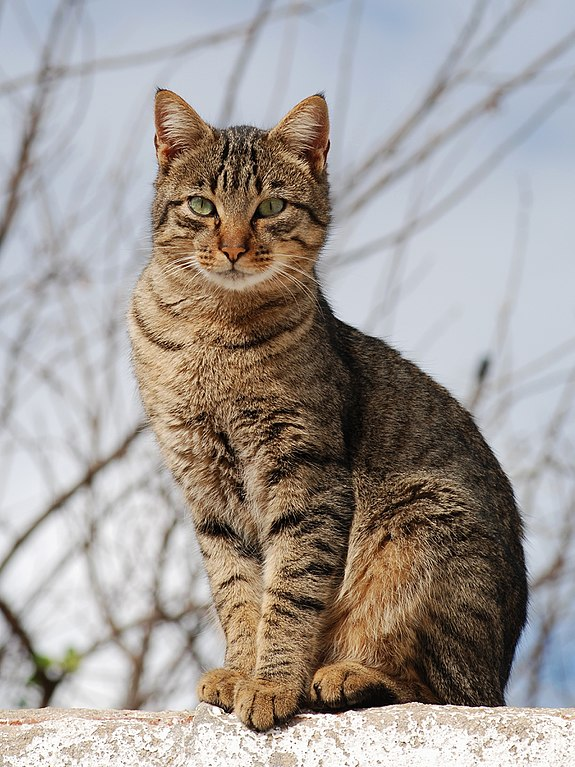
\includegraphics[width=0.31\textwidth]{media/cat}\nakedfootnote<2>{Wikipedia CC BY-SA 3.0}
    \centering
    \uncover<2>{
        \textbf{Cat}
    }
    \note[item]{For which photo would you ask the oracle for a label?}
    \note<2>[item]{Might learn to better use the eyes as a feature}
    \vspace*{\fill}
\end{frame}

\begin{frame}{Interventions resolve model underdetermination}
    \adjincludegraphics[width=\textwidth,trim={{.005\width} 0 0 0},clip]{media/opto-AL.jpg}
    \note{We discuss single neuron stim for intuition. For multi-neuron stim, easier to think in terms of latent space.}
\end{frame}{}

\begin{frame}{Bayesian Active Learning by Disagreement}
    We want to maximize the decrease in expected posterior entropy of model parameters:
    \begin{align}
        \argmax_{s_t} H[\theta|x_{1:t}] - \mathbf{E}_{x_{t+1}}[H[\theta|s_t,x_{t+1},x_{1:t}]]
    \end{align}
    Entropy of model parameters $\theta$ is intractable. So we rearrange to:
    \begin{align}
        \argmax_{s_t} H[x_{t+1}|s_t,x_{1:t}] - \mathbf{E}_{\theta}[H[x_{t+1}|s_t,x_{1:t},\theta]]
    \end{align}
    \nakedfootnote{Houlsby, Huszár, et al. 2011}
\end{frame}

\begin{frame}{Bayesian deep learning via dropout}
    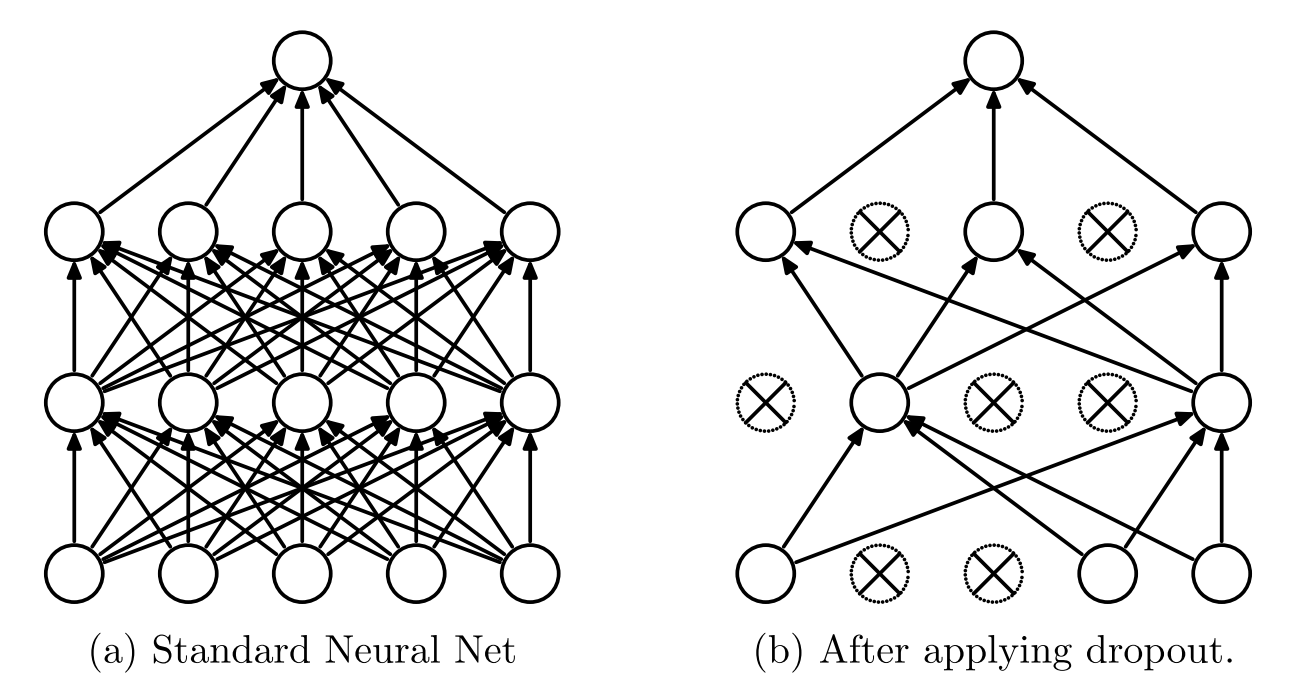
\includegraphics[width=\textwidth]{media/dropout}
    \nakedfootnote{Srivastava, Hinton, et al. 2014}
    \nakedfootnote{Gal 2016}
\end{frame}{}

\begin{frame}{ Collect data then iterate the approach offline }
    Data collection:
    \begin{itemize}
        \item [1] 180 trials of looming stimuli (1 hour)
        \item [2] 360 trials of random single-cell perturbation ( 1 hour)
        \item [3] 180 trials of looming stimuli (1 hour)
    \end{itemize}{}
    Data analysis:
    \begin{itemize}
        \item train on 80\% of trials from [1 \& 3]
        \item choose 60 trials from [2]
        \item Test on witheld trials from [1 \& 3]
    \end{itemize}{}
    How much better can we do by choosing trials vs random trials in terms of test performance?
    \note{This design is mainly to validate our choice of acquisition function (how we choose stimuli) as we can collect all data first then iterate on computational side}
\end{frame}{}

\begin{frame}{ Online optimal experiment design }
    Data collection:
    \begin{itemize}
        \item [1] 225 trials of looming stimuli (1 hour 15 min)
        \item [2] 360 trials, model chooses each single-cell perturbation ( 1 hour)
        \item [3] 225 trials of looming stimuli (1 hour 15 min)
    \end{itemize}{}

    How well can we predict test data by training on 2 hours of looming stimuli vs 1 hour looming \& 1 hour optogenetics?
    \note[item]{Once we've validated offline, can try online. How much can we condense model learning / improve performance?}
    \note[item]{Additional advantage of spatial model is no need for motion correction as convolution is translation invariant. Potential advantage over onACID (online CNMF).}
\end{frame}{}


\begin{frame}{ Brain state replay }
    Data collection:
    \begin{itemize}
        \item [1] Acquire brain trajectory of interest
        \item [2] choose each stimulation pattern sequentially during resting state / experiment of interest
        \item [3] Stim brain to keep observations in line with [1]
    \end{itemize}{}

    How well can we track a previously observed trajectory?

\end{frame}{}
